\documentclass{beamer}
\usetheme{metropolis}           % Use metropolis theme
\usecolortheme{beaver}
\setbeamerfont{caption}{size=\scriptsize}
\title{Charla GitHub avanzado 2024}
\subtitle{Ramas, comunicación, workflows}
\date{2024}
\author{Alejandro Barrachina Argudo}
\institute{Universidad Complutense de Madrid}
\begin{document}
\maketitle

\begin{frame}{Tabla de contenidos}
    \tableofcontents
\end{frame}

\AtBeginSection[]{
    \begin{frame}{Tabla de contenidos}
        \tableofcontents[currentsection]
    \end{frame}
}
\AtBeginSubsection[]{
    \begin{frame}{Tabla de contenidos}
        \tableofcontents[currentsubsection]
    \end{frame}
}
\section{Introducción}
\begin{frame}{Introducción}

    Charla anterior: \url{https://github.com/ALK222/charla-git-principiantes-2023}
    
    Se asume que:
    \begin{itemize}
        \item Tenéis cuenta de GitHub
        \item Sabéis hacer crear repositorios
        \item Sabéis hacer \textit{commit}, \textit{push}, \textit{pull}
    \end{itemize}
\end{frame}

\section{Ramas}
\begin{frame}{Ramas}
    \begin{itemize}
    \item Mantienen el desarrollo paralelo para distintas partes del programa

    \item Mantienen separadas las versiones estables de las de desarrollo
     
    \item Nos permiten proteger ciertas ramas
\end{itemize}

\end{frame}

\begin{frame}
    \begin{figure}[H]
        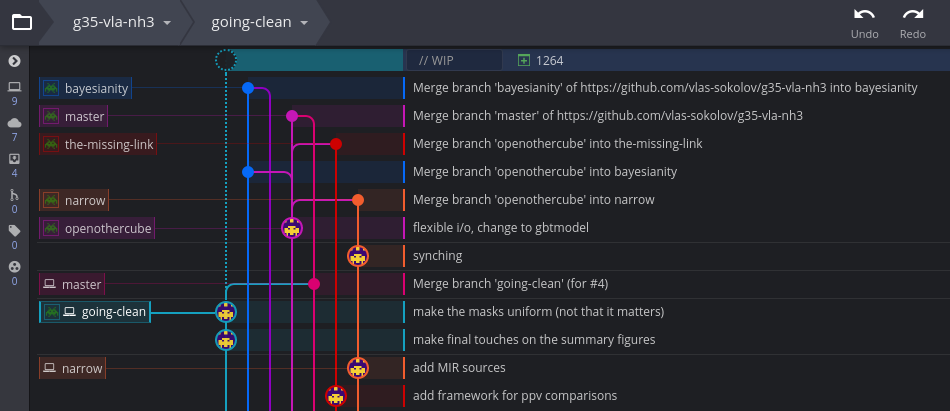
\includegraphics[width=0.7\textwidth]{Images/ejemplo-ramas.png}
        \caption{origen de la imagen: \url{https://stackoverflow.com/questions/46827112/toggling-branch-tree-view-in-gitkraken}}
    \end{figure}
\end{frame}
\subsection{Main}
\begin{frame}{Main}
    
    La rama Main (en proyectos antiguos también se puede encontrar como Master) es la rama principal del proyecto y la primera rama que se crea automáticamente al crear el repositorio.

    \begin{itemize}
        \item Rama (normalmente) protegida para evitar código malicioso (de manera intencional o no) sin supervisión.
        \item Generalmente es la rama estable del programa, solo se suben versiones definitivas
    \end{itemize}

\end{frame}
\subsection{Ramas secundarias}
\begin{frame}{Ramas secundarias}
    A estas ramas les daremos nosotros un nombre al crearlas. Son útiles para desarrollar nuevas características del programa o para hacer arreglos de bugs.

    Estas ramas se pueden unir a la principal en cualquier momento del desarrollo para incorporar estos cambios a la rama principal.
\end{frame}
\subsection{Pull request y Merge}
\begin{frame}{Merge}
    
    Un \textit{Merge} nos permite unificar un conjunto de \textit{commits} en un solo historial. 
    
    Normalmente esto se hace entre los extremos de dos ramas para fusionarlas en una sola.

    Esto puede generar conflictos entre archivos que se pueden resolver con distintos editores de texto o herramientas de gestión de git.

\end{frame}

\begin{frame}{Pull Request}

    Un \textit{pull request} es un mecanismo de GitHub para poder hacer \textit{merge} en proyectos ajenos o para solicitar feedback antes de hacer un merge en tu propio proyecto.

    En ciertos repositorios es obligatorio pasar una \textit{pull request} con varios supervisores para poder contribuir si no eres parte del equipo.

\end{frame}
\end{document}